% on bueler-leopard see
%   /usr/share/doc/latex-beamer/solutions/conference-talks/conference-ornate-20min.en.tex

\documentclass{beamer}

\usetheme{Pittsburgh}
\setbeamercovered{transparent}
\setbeamertemplate{navigation symbols}{} %remove navigation symbols

\usepackage[english]{babel}
\usepackage[latin1]{inputenc}

\usepackage{times}
\usepackage[T1]{fontenc}

% math macros
\newcommand\bb{\mathbf{b}}
\newcommand\bbf{\mathbf{f}}
\newcommand\bn{\mathbf{n}}
\newcommand\bq{\mathbf{q}}
\newcommand\bu{\mathbf{u}}
\newcommand\bv{\mathbf{v}}
\newcommand\by{\mathbf{y}}

\newcommand\bQ{\mathbf{Q}}
\newcommand\bV{\mathbf{V}}
\newcommand\bX{\mathbf{X}}

\newcommand\CC{\mathbb{C}}
\newcommand{\DDt}[1]{\ensuremath{\frac{d #1}{d t}}}
\newcommand{\ddt}[1]{\ensuremath{\frac{\partial #1}{\partial t}}}
\newcommand{\ddx}[1]{\ensuremath{\frac{\partial #1}{\partial x}}}
\newcommand{\ddy}[1]{\ensuremath{\frac{\partial #1}{\partial y}}}
\newcommand{\ddxp}[1]{\ensuremath{\frac{\partial #1}{\partial x'}}}
\newcommand{\ddz}[1]{\ensuremath{\frac{\partial #1}{\partial z}}}
\newcommand{\ddxx}[1]{\ensuremath{\frac{\partial^2 #1}{\partial x^2}}}
\newcommand{\ddyy}[1]{\ensuremath{\frac{\partial^2 #1}{\partial y^2}}}
\newcommand{\ddxy}[1]{\ensuremath{\frac{\partial^2 #1}{\partial x \partial y}}}
\newcommand{\ddzz}[1]{\ensuremath{\frac{\partial^2 #1}{\partial z^2}}}
\newcommand{\Div}{\nabla\cdot}
\newcommand\eps{\epsilon}
\newcommand{\grad}{\nabla}
\newcommand{\ihat}{\mathbf{i}}
\newcommand{\ip}[2]{\ensuremath{\left<#1,#2\right>}}
\newcommand{\jhat}{\mathbf{j}}
\newcommand{\khat}{\mathbf{k}}
\newcommand{\nhat}{\mathbf{n}}
\newcommand\lam{\lambda}
\newcommand\lap{\triangle}
\newcommand\Matlab{\textsc{Matlab}\xspace}
\newcommand\RR{\mathbb{R}}
\newcommand\vf{\varphi}


\title[Conservation in free-boundary layers] % (optional, use only with long paper titles)
{Conservation \\ in free-boundary fluid layer models}


\author{Ed Bueler}

\institute[UAF] % (optional, but mostly needed)
{
  Dept of Mathematics and Statistics, and Geophysical Institute\\
  University of Alaska Fairbanks%
}

\date{{\scriptsize AGU 2014}}


% If you have a file called "university-logo-filename.xxx", where xxx
% is a graphic format that can be processed by latex or pdflatex,
% resp., then you can add a logo as follows:
% \pgfdeclareimage[height=0.5cm]{university-logo}{university-logo-filename}
% \logo{\pgfuseimage{university-logo}}



% Delete this, if you do not want the table of contents to pop up at
% the beginning of each subsection:
%\AtBeginSection[]
%{
%  \begin{frame}<beamer>{Outline}
%    \tableofcontents[currentsection]
%    %\tableofcontents[currentsection,currentsubsection]
%  \end{frame}
%}


\begin{document}
\graphicspath{{../images/}{../../talks-public/commonfigs/}}

\begin{frame}
  \titlepage
\end{frame}

\begin{frame}{Outline}
  \tableofcontents
\end{frame}


% Structuring a talk is a difficult task and the following structure
% may not be suitable. Here are some rules that apply for this
% solution: 

% - Exactly two or three sections (other than the summary).
% - At *most* three subsections per section.
% - Talk about 30s to 2min per frame. So there should be between about
%   15 and 30 frames, all told.

% - A conference audience is likely to know very little of what you
%   are going to talk about. So *simplify*!
% - In a 20min talk, getting the main ideas across is hard
%   enough. Leave out details, even if it means being less precise than
%   you think necessary.
% - If you omit details that are vital to the proof/implementation,
%   just say so once. Everybody will be happy with that.

\section{The problem}

\subsection{Free-boundary fluid layer well-posedness.}

\begin{frame}{A fluid layer in a climate}

\begin{center}
\only<1>{\includegraphics[width=\textwidth,keepaspectratio=true]{cartoon-layer}}
\only<2->{\includegraphics[width=\textwidth,keepaspectratio=true]{cartoon-wclimate}}
\end{center}

\vspace{-9mm}
  \begin{itemize}
  \item mass conservation for a layer:
     \only<1>{$$h_t + \Div\bq = f$$}
     \only<2->{$$h_t + \Div\bq = {\color{blue} f}$$}
    \begin{itemize}
    \vspace{-4mm}
    \item<1->[$\circ$] mass conservation PDE applies \emph{only where} $h>0$
    \item<2->[$\circ$] source ${\color{blue} f}$
    \item<2->[$\circ$] $f>0$ shown downward (accumulation)
    \end{itemize}
  \item<3> $h$ is a thickness:
      $$h\ge 0$$
  \end{itemize}
\end{frame}


\begin{frame}{A fluid layer in a climate (\emph{difficulties})}

\begin{center}
\only<1>{\includegraphics[width=\textwidth,keepaspectratio=true]{cartoon-sensitive-one}}
\only<2>{\includegraphics[width=\textwidth,keepaspectratio=true]{cartoon-sensitive-two}}
\only<3>{\includegraphics[width=\textwidth,keepaspectratio=true]{cartoon-sensitive-three}}
\end{center}

\vspace{-18mm}
$$h_t + \Div\bq = {\color{blue} f}$$

  \begin{itemize}
  \item<1-> $f<0$ not ``detected'' by model where $h=0$
     \begin{itemize}
     \item<1->[$\circ$] how to do mass conservation accounting?
     \end{itemize}
  \item<2-> $f\approx 0$ threshold behavior
     \begin{itemize}
     \item<2->[$\circ$] $h>0$ as soon as $f<0$ switches to $f>0$
     \end{itemize}
  \item<3> $h=0$ \emph{and what else} at free boundary?
     \begin{itemize}
     \item<3>[$\circ$] shape of free boundary depends on flux $\bq$
     \end{itemize}
  \end{itemize}
\end{frame}


\begin{frame}{Examples}

\includegraphics[width=0.42\textwidth,keepaspectratio=true]{polaris}
\hfill
\includegraphics[width=0.47\textwidth,keepaspectratio=true]{supp4rignot-small}

\small glaciers \hfill ice shelves \& sea ice

\medskip
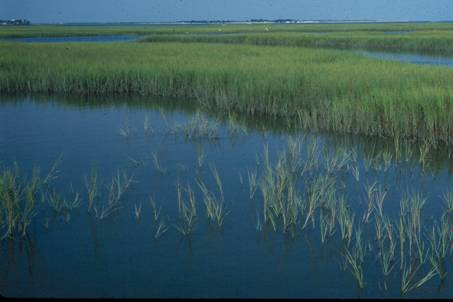
\includegraphics[width=0.43\textwidth,keepaspectratio=true]{marsh-water}
\hfill
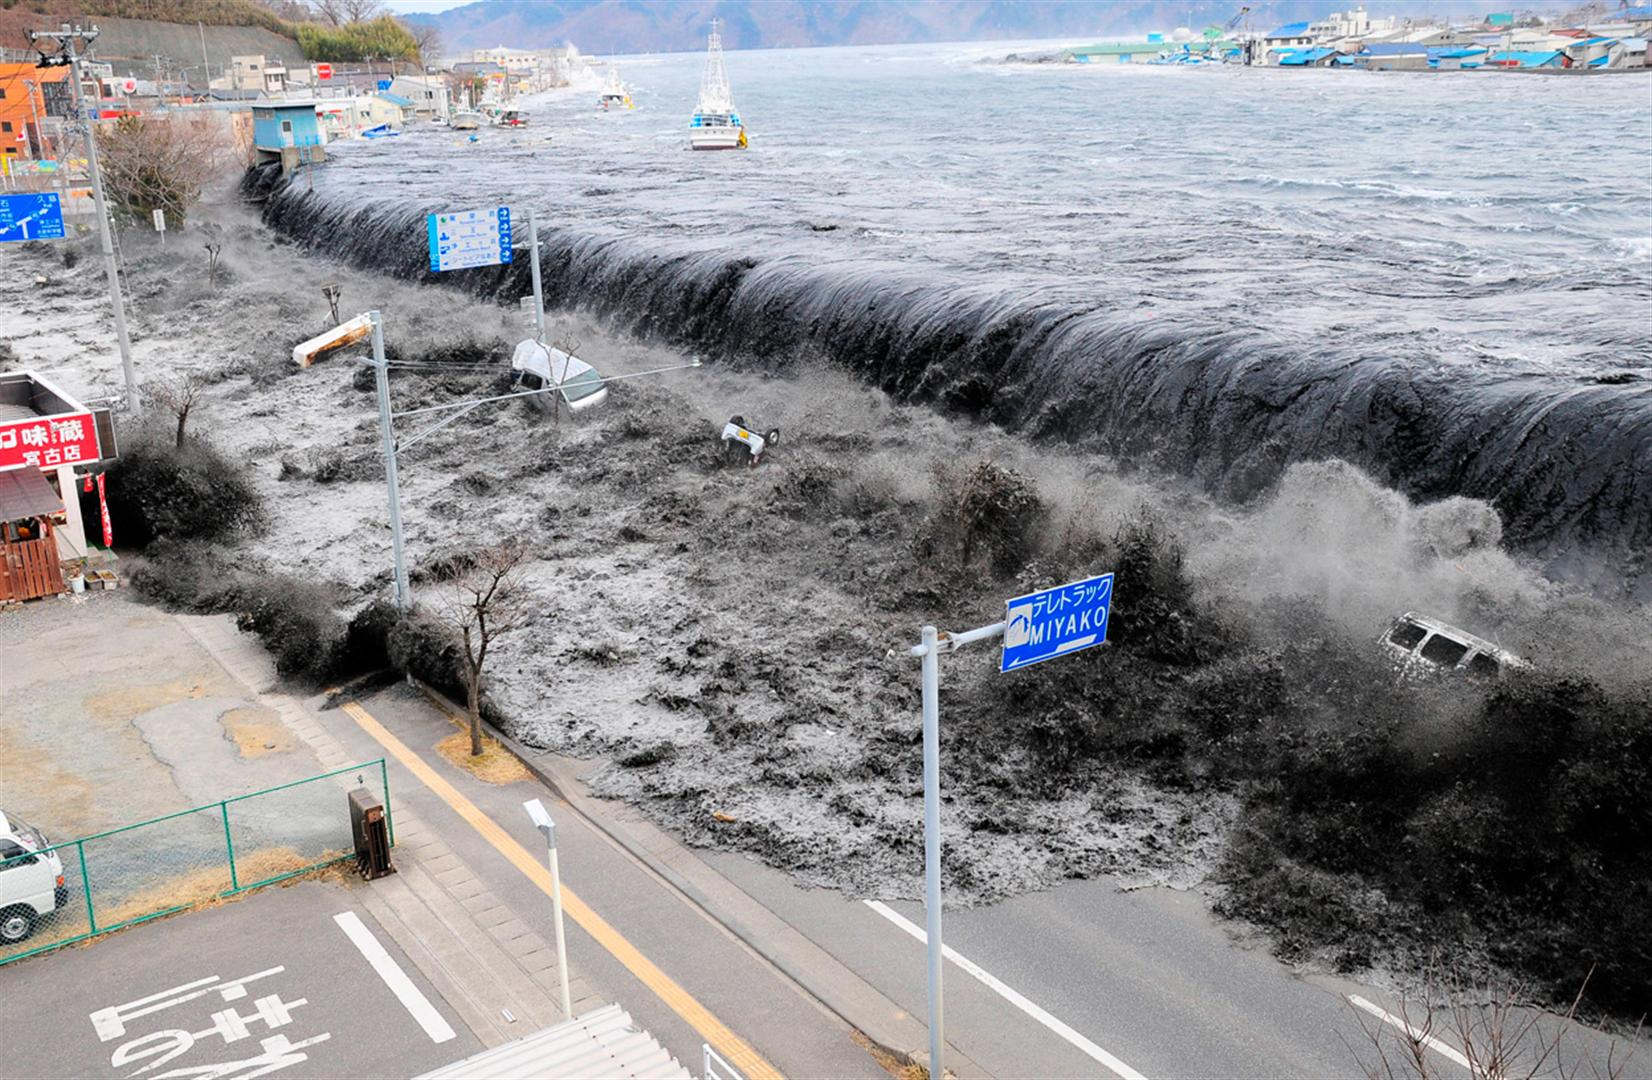
\includegraphics[width=0.44\textwidth,keepaspectratio=true]{tsunami-sendai}

\small tidewater marsh \hfill tsunami inundation

%\vspace{-2mm}
%{\tiny {\color{gray} (Alonso, Santillana \& Dawson, 2008)}}

\medskip
\scriptsize and subglacial hydrology, supraglacial runoff, general surface hydrology, \dots


\end{frame}


\begin{frame}{Numerical models \emph{must} discretize time}

$$h_t + \Div\bq = f \qquad \to \qquad \frac{H_n - H_{n-1}}{\Delta t} + \Div \bQ_n = F_n$$

  \begin{itemize}
  \item semi-discretize in time
    \begin{itemize}
    \item[$\circ$] $H_n\ge 0$ is the thickness at $t_n$
    \item[$\circ$] new equation is PDE in space (where $H_n>0$)
    \item[$\circ$] I'll call it the ``single time-step problem''
    \end{itemize}
  \item flux $\bQ_n$ depends on $H_n,\grad H_n,x$
  \item source $F_n$ depends on $H_n,H_{n-1},x$
  \item<2-> details of $\bQ_n$, $F_n$ from time-step scheme
    \begin{itemize}
    \item<2->[$\circ$] forward/backward Euler, trapezoid, RK all o.k.
    \end{itemize}
  \item<3> low regularity of $h(t,x)$ for $x$ near margin means low accuracy expectations for time-step scheme
  \end{itemize}
\end{frame}


\begin{frame}{Anyone faced these problems before?}

  \begin{itemize}
  \item yes, of course!  for example:
    \begin{itemize}
    \item[$\circ$] ad hoc schemes for finite volume/difference mass conservation
    \end{itemize}
  \only<2>{\item I don't mind ``\texttt{if \dots then \dots}'' in my code
  \item \emph{but I want to know what mathematical problem it reflects!}}
  \end{itemize}

\only<1>{
\begin{columns}
\begin{column}{0.3\textwidth}
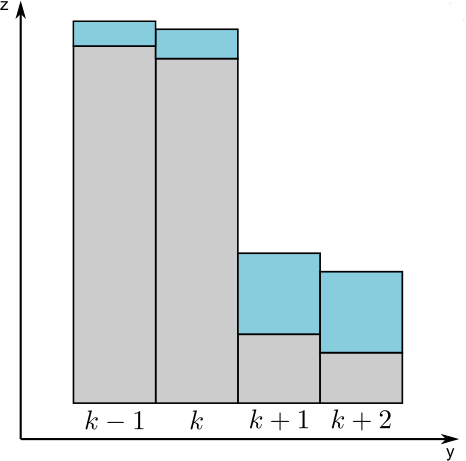
\includegraphics[width=\textwidth,keepaspectratio=true]{JaroschSchoofAnslow2013}

\small glacier ice

on steep terrain

\smallskip
\tiny (Jarosch, Schoof, Anslow, 2013)
\end{column}

\begin{column}{0.6\textwidth}
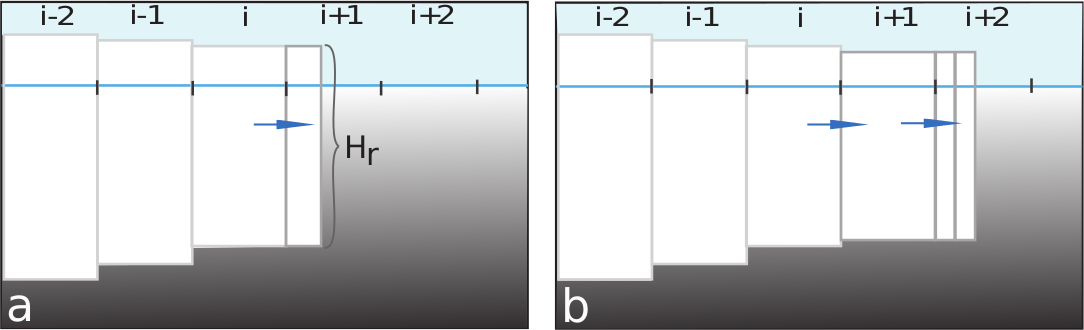
\includegraphics[width=0.8\textwidth,keepaspectratio=true]{Albrechtetal2011}

\small ice shelf fronts

\tiny (Albrecht et al, 2011)

\small \medskip
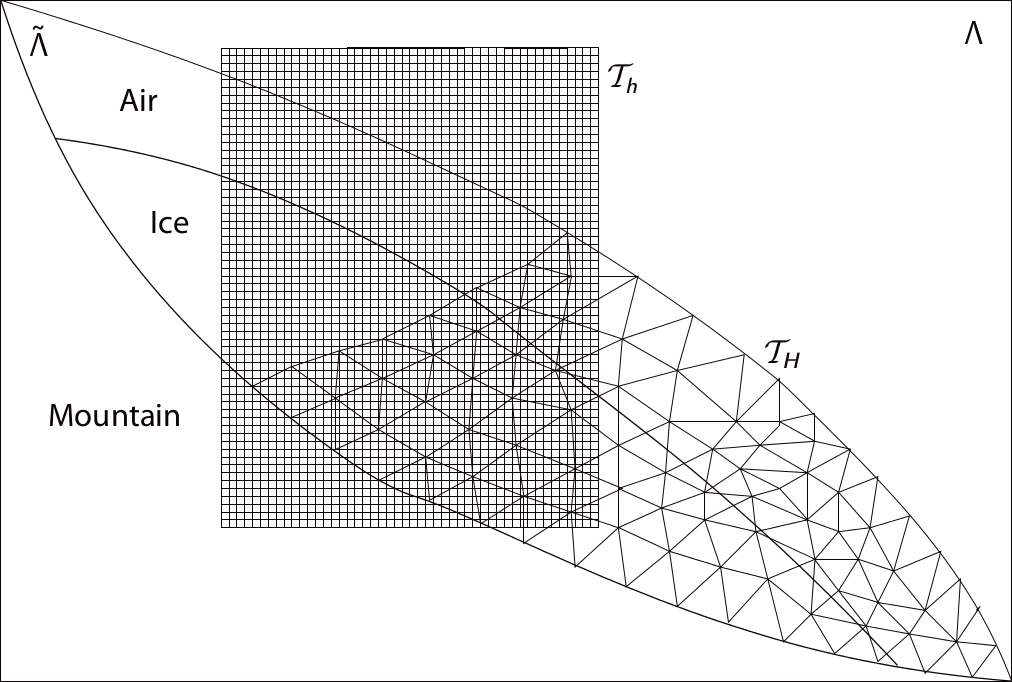
\includegraphics[width=0.6\textwidth,keepaspectratio=true]{jouvet-two-grids}

\small volume-of-fluid method on fine grid

\tiny (Jouvet et al 2008)
\end{column}
\end{columns}}

\only<2>{\phantom{foo}

\vspace{38mm}
\phantom{bar}}
\end{frame}


\begin{frame}{Weak form includes $h\ge 0$ constraint}

  \begin{itemize}
  \item equation \,$\frac{H_n - H_{n-1}}{\Delta t} + \Div \bQ_n = F_n$\, is single time-step ``strong form''
  \item closed convex set of admissible thicknesses $H_n$:
    $$FIXME define \mathcal{K}$$
  \item
    $$FIXME state VI$$
  \end{itemize}
\end{frame}


% could put this in
%\begin{frame}{Decomposition into sets}
%\end{frame}


\section{What's achievable?}

\subsection{Limits to auditable discrete conservation.}

\begin{frame}{FIXME}
\end{frame}


\section*{Summary}

\begin{frame}{Summary}

  % Keep the summary *very short*.
  \begin{itemize}
  \item
    The \alert{first main message} of your talk in one or two lines.
  \item
    The \alert{second main message} of your talk in one or two lines.
  \item
    Perhaps a \alert{third message}, but not more than that.
  \end{itemize}
  
  % The following outlook is optional.
  \vskip0pt plus.5fill
  \begin{itemize}
  \item
    Outlook
    \begin{itemize}
    \item
      Something you haven't solved.
    \item
      Something else you haven't solved.
    \end{itemize}
  \end{itemize}
\end{frame}


\end{document}


